\documentclass[12pt,a4paper]{article}
\usepackage[utf8]{inputenc}
\usepackage[T1]{fontenc}
\usepackage[english]{babel}
\usepackage{parskip}
\usepackage{graphicx}
\usepackage{url}
\title{Checkers in Haskell}
\author{By: Daniel Jönsson, Madelene Alanenpää, Henrik Schulze }
\date{PKD 2017 - 2018}
\begin{document}
\maketitle
\newpage
\tableofcontents
\newpage

\section{Introduction}
After some discussions on what project to do we decided to make the game checkers in Haskell. Our programme lets two users play checkers in Haskell against each other. 

Checkers is an old game that can be played on a chessboard or on a bigger board. We decided to implement it on a chessboard with 8*8 squares. The rules can vary quite alot in checkers but the following rules are what we worked from. All the 12 pieces on each side of the board stand on the dark squares in the first 3 rows when the game starts. Below is an example of a starting board for checkers.

\begin{center}
	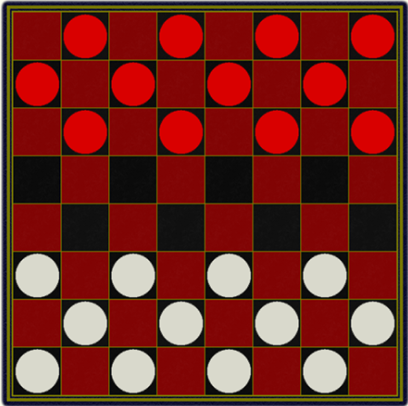
\includegraphics[width= 0.3\textwidth]{Startboarexample.PNG}	
\end{center}


In checkers pieces always move diagonally so they will stay on the black squares durning the whole game. A piece making a non-capturing move (not involving a jump) may move only one square in a forward direction. A piece making a capturing move (a jump) stands next to an opponent and leaps over that opponent landing in a straight diagonal line on the other side. The jump can only be made if the square after the opponent is empty so only one piece may be captured in a single jump. Multiple jumps with one piece should be made if that is possible during a single turn. The pieces can jump in both directions when capturing opponents.

When a piece is captured, it is removed from the board. If a player can make a capture, there is no option; the jump must be made. If captures are available for several pieces, the player is free to jump with whichever he or she prefers. When a piece reaches the furthest row from the player who controls that piece, it is crowned and becomes a king. A king has more freedom and can move several steps in a diagonal line if the line is free. When a king makes a jump, it can make it if the space behind the opponent is free even if the king is not standing next to that piece.

\section{Summary}
So, what did we accomplish with our code? 

We feel satisfied with our work since we managed to make a functional game in Haskell where it is possible for two human players to play checkers. The game follows the rules of checkers as described in the introduction with some small exceptions that are described in section 5. 


Pieces are put out diagonally on the first three lines of the board and from here they can only move  diagonally. When the game starts it is only possible for the red player to move, then the players take turns. Pieces can only move one step forward unless they have the possibility to make one or several jumps. They can’t jump outside the board and a piece will be removed once it has been jumped over. If a piece have made a jump and can make another one it has to make that jump. When a piece moves all the way to the "end" of the board it will be transformed to a queen. A player loses the game when he/she has no more pieces left on the board.

The game prints out a new updated board after every move. Our code will check if a move is valid so it is not possible to make a move that is not allowed.

\section{Usage of Program}
To start our program you first need a Haskellplatform with GHCI. This you can download at https://www.haskell.org/platform/ for Windows, Linux and Mac OS X. When the installation is finished in Windows start WinGHCi and load Checkers.hs. In Mac OS X run the installer, follow the instructions and then open Checkers.hs. For Linux follow the instructions on the webpage and then open Checkers.hs.
\newpage
When you have loaded Checkers.hs write main and press enter. Now you will get a starting board as below. From here you can start to play. 		

\begin{center}
	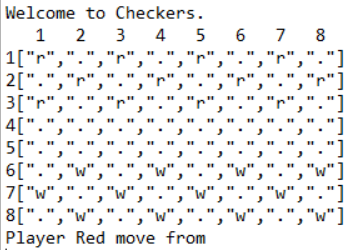
\includegraphics[width= 0.4\textwidth]{start.PNG}
\end{center}

To start you write a tuple with two numbers that represents from where you want to move and press enter. Then you write a new tuple representing where you want to move and press enter again. The first number in the tuple represents the row and the second represents the column. Look at example below.


Player Red move from

(3,1)

Player Red move to

(4,2)

Player Red moves from  (3,1)  to  (4,2)

Now you will get an updated board with the move applied as you can see below,

\begin{center}
	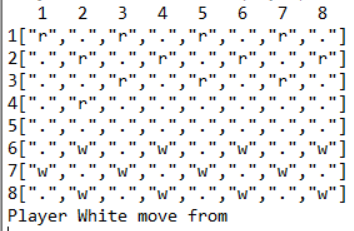
\includegraphics[width= 0.4\textwidth]{firstmove.PNG}
\end{center}
it will be whites turn and like this it continues. 
\newpage
To jump over another player you write your "starting coordinates" as usual and the "move to coordinates" behind the player to jump. The board will then be updated with your piece on the new position and the piece you jumped will be removed. If you have possiblity to make a jump with more than one piece you can choose which  piece you want to jump with. A jump can look something like this below where red jumps from position (4,2) to (6,4).

\begin{center}
	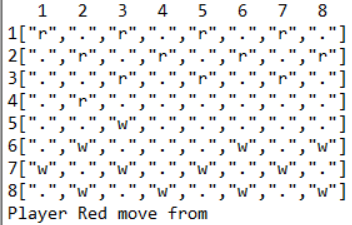
\includegraphics[width= 0.4\textwidth]{jump1.PNG}    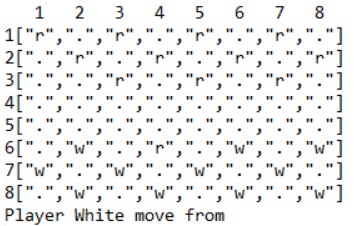
\includegraphics[width= 0.4\textwidth]{jump2.PNG} 
\end{center}

If you have possibility to make several jumps with one piece you have to do that once you have made the first jump. You make the first jump as usual and a new board will be printed. Now you need to make another jump and you can not move another piece. You make the next jump in the same way as any other jump. In the pictures below you can see how the red player makes multiple jumps from position (4,4) to (6,6) and from (6,6) to (8,8) before it is whites turn.

\begin{center}
	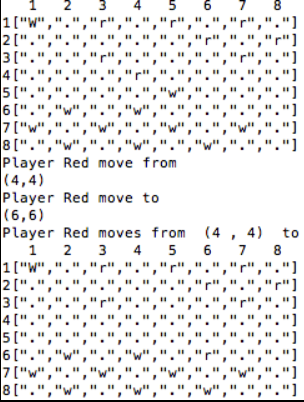
\includegraphics[width= 0.4\textwidth]{mj1.PNG} 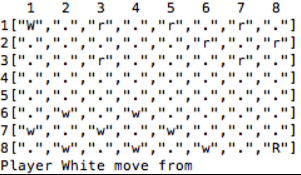
\includegraphics[width= 0.4\textwidth]{mj2.PNG}
\end{center}


If a player moves over the board to the other side it will be upgraded to a queen and that will be represented with a capital r or a capital w, see next page where a red piece have moved to the other side, position (8,6).

\begin{center}
	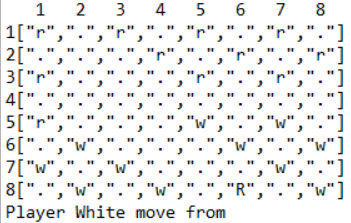
\includegraphics[width= 0.4\textwidth]{queen.PNG}
\end{center}

A player wins when the opponent have no more pieces on the board and then you can choose if you want to quite or continue. The end board can look like this.

\begin{center}
	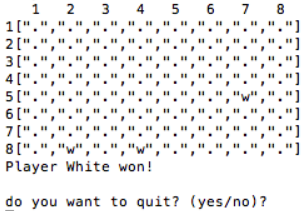
\includegraphics[width= 0.4\textwidth]{victory.PNG}
\end{center}

If you write a move that is invalid you will get a message that says something like this.

\textit{"Player Red moves from (3 , 1) to (1 , 4)
Invalid Move. You can only move your own pieces and move diagonally"}

\textit{"Player Red move from"}

If you write your move in the wrong format you will get a message that says 

\textit{"Invalid input. Correct format: (row,column)"}




\section{Program Documentation}
\subsection{Description of data structures}
The data types on the next page are the ones we have defined and use for our checkers game in Haskell. As described earlier in the report the pieces in Checkers are either kings or a pawns that are red or white so we needed some data types that could help us represent this on our board.
\newpage\textbf{data Player = Player Color Type}

\textbf{data Color = Red | White}

\textbf{data Rank?? = Normal | King}

Since we made our empty board as a list of 64 ".", we didn't need to have data types for representing "." on the board. In the code we use our data types in functions that reads and shows our Players, see below. 


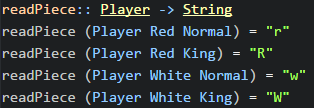
\includegraphics[width= 0.4\textwidth]{read.PNG}  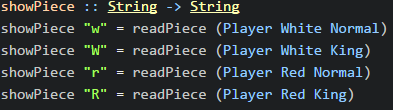
\includegraphics[width= 0.5\textwidth]{show.PNG}

We use read- and showPiece in different funtions in our code like in insertPlayer where we use readPiece.

\subsection{Description of algorithms and functions}
\textbf{\large {main}}
\\
Description: Generates the starting board for the players and prints it out in the terminal.
It also displays the message "Welcome to Checkers"
\\

\section{Known Shortcomings}
We did not manage to implement all the things that we had as goals such as creating a computer player and making the game available with Gloss graphics.
Our initial idea was to make the game in a few steps in Haskell. We would first make it so that two players could play against each other, then create a computer player that would be able to play in a simple way against a human and to implement gloss graphics for our game. It was a challenge to make the game so that two players could play against each other, so we decided only to stop after that since we didn’t have enough time to also implement a computer player. We also had some problems with implementing the gloss graphics in the game.

\end{document}
